\section{Analysis of Gas in the Australian National Electricity Market}

In this section we will be taking a closer look at the significance of Gas in Australia’s Domestic National Electricity Market (NEM). The NEM is one of the biggest distributed energy systems in the world and is the deregulated portion of Australian energy, and hinges on an efficient market. We will conduct our study on Gas consumption price to national average spot energy price and compared to other means of electricity generation, this will be done using Multivariable Vector Autogregression model (MVAR) and using quantity consumed and average spot prices.

\subsection{Observations}

Energy consumption data in NEM is gathered from AEMO \cite{NEM1} combined with OpenNEM \cite{NEM2} is categorized by the top 11 energies consumed:

\begin{multicols}{4}
\begin{itemize}
    \item Battery (Discharging)
    \item Wind
    \item Solar (Utility)
    \item Solar (Rooftop)
    \item Hydro
    \item Coal (Brown)
    \item Coal (Black)
    \item Gas (Steam)
    \item Gas (CCGT)
    \item Gas (OCGT)
    \item Gas (Reciprocating)
\end{itemize}
\end{multicols}

\begin{figure}[H]
    \centering
    \subfloat[\centering Stacked Barplot of GigaWatt hours energy consumed ]{{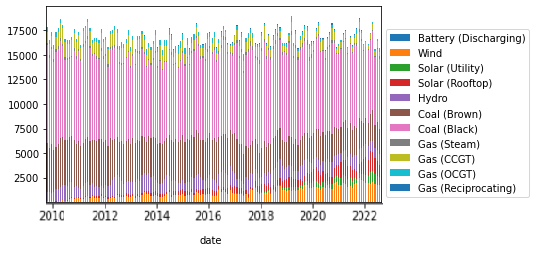
\includegraphics[width=0.4\textwidth]{Figures/NEM-Analysis/consumption.png} }}%
    \qquad
    \subfloat[\centering Price of each energy per GigaWatt ]{{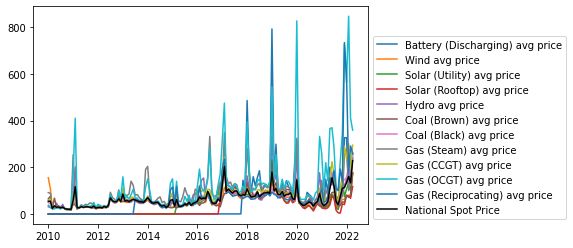
\includegraphics[width=0.4\textwidth]{Figures/NEM-Analysis/price_gigawatt.png} }}%
    \caption{figures for every month 2009-2022}%
    \label{fig:NEM-consump-price}%
\end{figure}

As a general overview, we can see there is cyclical pattern of aggregate consumption where the barplot display a cyclical pattern, this is different to global analyses and could be because of physical weather and seasons. Another observation is the use of Hydrocarbons (such as gas and coal) generally decreasing over time, which is opposite to renewable energies, particularly wind and solar, which are growing over time.
\medskip

Some particular observations are that different states have varying reliance on gas, for example Tasmania, which has so much excess supply of hydro electricity that it will export it to the NEM where it can be sold. Another observation is how South Australia's reliance on gas has decreased over time: in October 2009 it accounted for 61\% of the state's consumption but recently as of April 2022 it accounts for 20\%, compared to its renewable energy (combined Solar and Wind) consumption which accounts for 62\%.

\subsection{Data Preparation}

Though it is interesting to see specific observations like in our previous section, we will be using average spot prices as we are looking for significant systematic effects rather than special local cases.
\medskip

Since in figure \ref{fig:NEM-consump-price}.b, we observe that some Gas prices are 0 until 2018, we will focus from 2018 until present. We will also aggregate the different types of gas and combine their market value and energy consumption to model the aggregate effect of gas compared to the other energies. 
\medskip

To compare the impact of each energy source in the market we first need to convert each energy to its average spot price which we do by dividing aggregate market value and aggregate market consumption in terms of Australian Dollar per MegaWatt hours: 

\begin{equation*}
    \text{Average Energy Spot Price}=\frac{\text{Aggregate Energy Market Value}}{\text{Aggregate Energy Market Consumption}}
\end{equation*}
\medskip

After this is done, the energies prices are now comparable to each other. For the Vector Autoregression model to be fitted well, we need to enforce weak stationarity. For each energy timeseries, we attempted to enforce weak stationarity by normalizing subtracting its mean and divided by its standard deviation, and noticed yearly variance thus divided every year by its yearly variance to remove unfavourable seasonal volatility.

\begin{figure}[H]
    \centering
    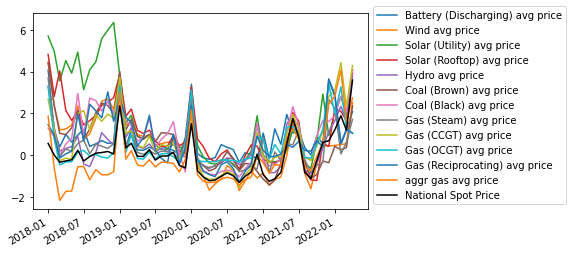
\includegraphics[width=0.6\textwidth]{Figures/NEM-Analysis/prep_data.png}
    \caption{Prepared Average spot price for each energy every month 2018-2022}
    \label{fig:NEM-avg-price}
\end{figure}

\subsection{Multivariate Vector Autoregression and Discussion}

Firstly, we run a Partial autocorrelation on national spot energy price to decide how many lags we should focus on. We find an AR(13) model with strong seasonality especially with 12th lag, this makes sense as last year's physical weather and season would be the most similar and thus, most significant.

\begin{figure}[H]
    \centering
    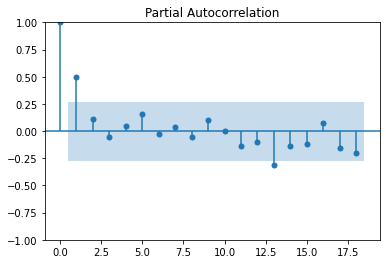
\includegraphics[width=0.6\textwidth]{Figures/NEM-Analysis/PACF-national.png}
    \caption{PACF of National Energy Spot Price}
    \label{fig:NEM-avg-price}
\end{figure}

Since we know NEM spot pricing is composed of the energies of interest, they are endogenous, and can be used to be modelled by a Multivariable Vector Autogregression model (MVAR). The function we run optimizes over AIC and BIC information criterion and gives us the following correlation matrix of residuals:

\begin{figure}[H]
    \centering
    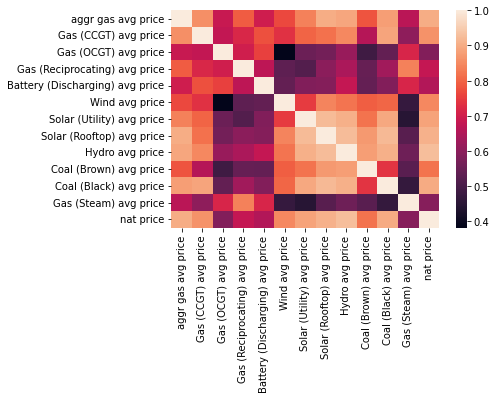
\includegraphics[width=0.6\textwidth]{Figures/NEM-Analysis/correl_var.png}
    \caption{Correlation Matrix of Residuals}
    \label{fig:NEM-correl}
\end{figure}

Observing results gives us a big MVAR model, which is overparameterized and not very useful for further prediction. However, we can compare relative effectiveness of each energy to each other. The correlation residuals show that national spot energy price has the highest correlation with Hydro and Solar Rooftop energy, but Lowest correlation with Gas STEAM and Gas OCGT. However, the spot price has a moderately high correlation to Aggregate gas pricing. This could be because gas STEAM is highly efficient but hard to provide consumption on demand, which is opposite to Gas OCGT where it is less efficient, but generators can be turned on almost instantly. Since these are aggregated, they provide a hedge to each other thus following the national spot price more closely.
\medskip

In this ad hoc MVAR analysis we find that individual gas price is not a great predictor of national spot price and aggregate gas spot price is only moderately correlated. Thus, international gas price fluctuations will have very minimal direct effect on domestic electricity generation from gas. Further analysis and more intensive modelling, perhaps incorporation of weather and seasonal data is required for more conclusive results.